\vbox to \myposterheight{%
\begin{block}{Experimental setup}
	\begin{itemize}
		\item Data acquisition:
		\begin{itemize}
			\item \textit{In-vitro} hyperechoic inclusion phantom~(Model 54GS, CIRS Inc., Norfolk, USA) and \textit{in-vivo} carotids
			\item Data acquired with a Verasonics research scanner~(V1-128, Verasonics Inc., Redmond, WA)
			\item ATL L12-5~\SI{50}{\milli\metre} ultrasound probe used for the different experiments
			\begin{itemize}
				\item \num{128} active transducer-elements
				\item \SI{5}{\mega\hertz} central frequency with \SI{100}{\percent} bandwidth
				\item \SI{31.2}{\mega\hertz} sampling frequency
			\end{itemize} 
			\item Transmission of plane waves with normal incidence
		\end{itemize}
		\item US-CMUX architecture 
		\begin{itemize}
			\item Simulated on MATLAB\textsuperscript{\textregistered}
			\item \num{2} cases: L=2 and L=4 
			\item Parameters of the reconstruction algorithm: $\epsilon = 10^{-6} \| \mathsf{Y}\|_F$, \num{1500} iterations
		\end{itemize}
		\item Image reconstruction:
		\begin{itemize}
			\item Achieved with standard delay-and-sum algorithm
			\item Post-processing pipeline for B-mode image
			\begin{itemize}
				\item Envelope extraction: Hilbert transform
				\item Normalization and log-compression with a dynamic range of \SI{40}{\decibel} 
			\end{itemize}
		\end{itemize}
	\end{itemize}
\end{block}
\vfill
%----------------------------------------------------------------------------------------
%	RECONSTRUCTED IMAGES
%----------------------------------------------------------------------------------------

\begin{block}{Reconstructed B-mode images}
	
	\newlength{\CIRSFigWidth} \setlength{\CIRSFigWidth}{0.24\textwidth}
	\newlength{\CIRSFigHeight}
	\settoheight{\CIRSFigHeight}{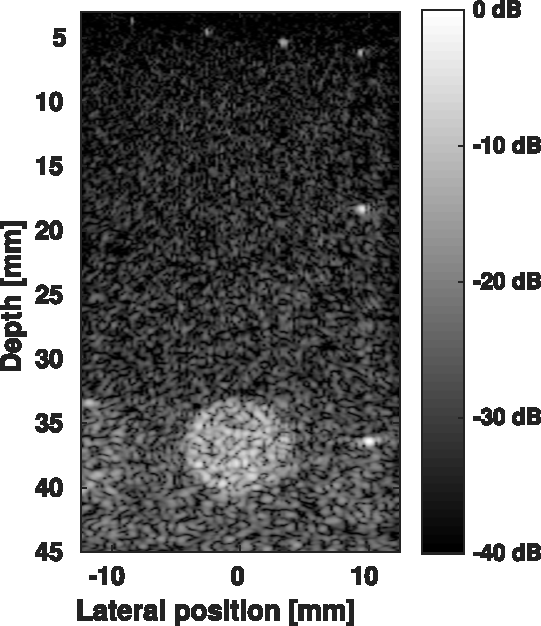
\includegraphics[width=\CIRSFigWidth]{figures/CS_hyperechoic.pdf}}
	\newlength{\CarotidFigWidth} \setlength{\CarotidFigWidth}{0.24\textwidth}
	\newlength{\CarotidFigHeight}
	\settoheight{\CarotidFigHeight}{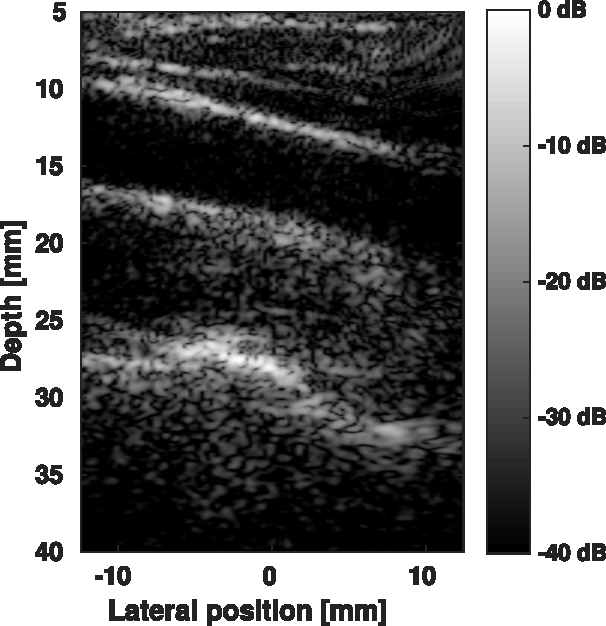
\includegraphics[width=\CarotidFigWidth]{figures/Reference_carotid.pdf}}  
	\begin{figure}
		\centering
		% Maximum length
		\subcaptionbox{Reference }{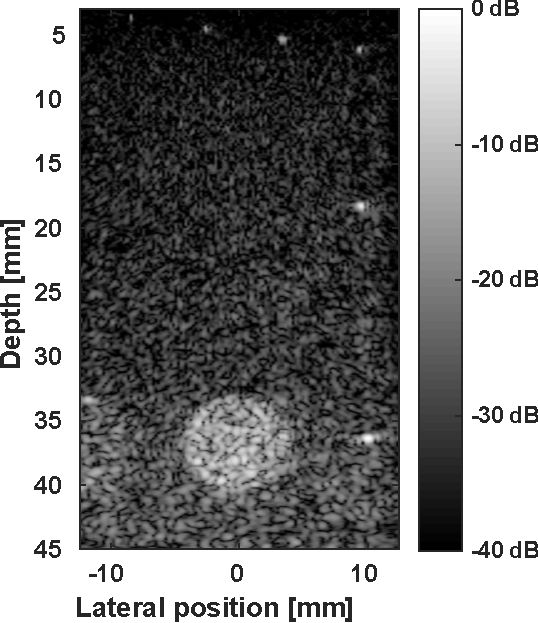
\includegraphics[height=\CIRSFigHeight]{figures/Reference_hyperechoic.pdf}}
		\subcaptionbox{CS reconstruction }{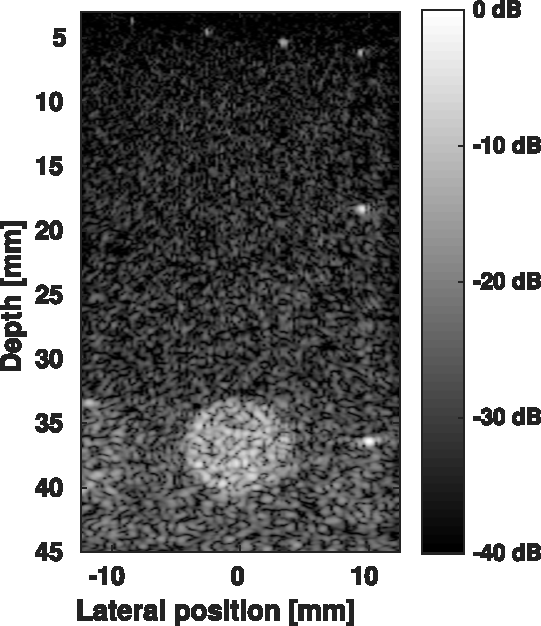
\includegraphics[height=\CIRSFigHeight]{figures/CS_hyperechoic.pdf}}
		\subcaptionbox{Reference }{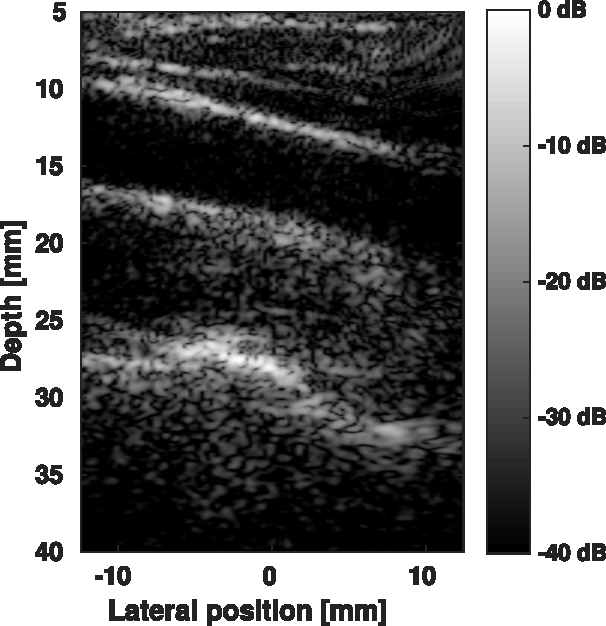
\includegraphics[height=\CarotidFigHeight]{figures/Reference_carotid.pdf}}
		\subcaptionbox{CS reconstruction }{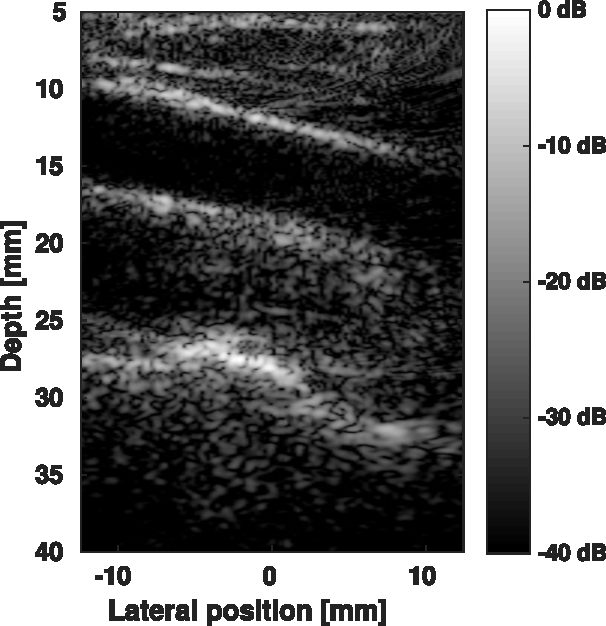
\includegraphics[height=\CarotidFigHeight]{figures/CS_carotid.pdf}}
		\caption{B-mode images of the hyperechoic inclusion and the carotid reconstructed with \SI{100}{\percent} of the data~((a) and (c)) and with \SI{25}{\percent} of the data acquired with US-CMUX~((b) and (d))}
	\end{figure}
	
\end{block}
\vfill
%----------------------------------------------------------------------------------------
%	IMAGE QUALITY METRICS
%----------------------------------------------------------------------------------------
\begin{block}{Quality metrics of the reconstructed images}
	\begin{itemize}
		\item PSNR and SSIM against B-mode images reconstructed with \SI{100}{\percent} data
	\begin{table}[htb]
		\caption{Average PSNR~$\left[\si{\decibel}\right]$ and SSIM~$\left[-\right]$ over \num{10} draws for the different images}
		\label{tab:SNR_SSIM}
		\centering
		\begin{tabular}{|c |c c|}
			\hline
			& Hyperechoic inclusion & \textit{In-vivo} carotid\\
			\hline
			PSNR - $L = 2$ & $39$ & $36$\\
			SSIM - $L = 2$ & $0.94$ & $0.87$\\
			PSNR - $L = 4$ & $32$ & $29$ \\
			SSIM - $L = 4$ & $0.81$ & $0.72$\\
			\hline
		\end{tabular}
	\end{table} 
		\item High quality reconstruction with \SI{25}{\percent} of the data.
	\end{itemize}
\end{block}
\vfill
%----------------------------------------------------------------------------------------
%	CONCLUSION
%----------------------------------------------------------------------------------------
\begin{block}{Conclusion and perspectives}
	\begin{enumerate}
		\item We propose a compressed sensing approach for US image recovery
		\begin{itemize}
			\item Exploits a stream of pulses model for sparsity of US images
			\item Uses multiple CMUX for analog compression of the data
			\item Applies a $\ell_{11}$-minimization algorithm for image reconstruction
		\end{itemize}
		\item The proposed approach leads to high-quality reconstruction with far fewer data than standard approaches
		\item Study of the hardware implementation will be achieved in future work
	\end{enumerate}
\end{block}
\vfill
%----------------------------------------------------------------------------------------
%	BIBLIOGRAPHY
%----------------------------------------------------------------------------------------
\begin{block}{References}
	\printbibliography
\end{block}
\vfill
%----------------------------------------------------------------------------------------
%	ACKNOWLEDGMENTS
%----------------------------------------------------------------------------------------
\begin{block}{Acknowledgments}
	This work was supported in part by the UltrasoundToGo RTD project (no. 20NA21 145911), evaluated by the Swiss NSF and funded by Nano-Tera.ch with Swiss Confederation financing.The authors would like to thank Dr~Olivier Bernard from CREATIS laboratory for providing the \textit{in vitro} and \textit{in vivo} acquisition data.
\end{block}
}%